\documentclass{beamer}
\usetheme{metropolis}

\title{Learning Contact Dynamics with LCP Constraint Relaxations}
\author{Samuel Pfrommer, Michael Posa}
\institute{DAIR Lab at the University of Pennsylvania}
\date{\today}

\usepackage{tikz}
\usetikzlibrary{arrows}
\usetikzlibrary{arrows.meta}
\usetikzlibrary{patterns,snakes}
\usetikzlibrary{calc}

\usepackage{caption}

\usepackage{listings}

\begin{document}

\lstset{language=C++,
    basicstyle=\ttfamily,
    keywordstyle=\color{blue}\ttfamily,
    stringstyle=\color{red}\ttfamily,
    commentstyle=\color{black!50!green}\ttfamily,
    morecomment=[l][\color{magenta}]{\#}
}

\begin{frame}
    \titlepage
\end{frame}

\begin{frame}
    \frametitle{Overview}
    \begin{itemize}
        \item Problems with manipulation
        \item Existing approaches
        \item How are we learning?
        \item What are we learning?
    \end{itemize}
\end{frame}

\begin{frame}
    \frametitle{Problems with manipulation}
    \begin{itemize}
        \item Sudden changes in dynamics when making/breaking contact 
        \item Inconsistencies with Coulomb friction (Painlev\'{e} paradox)
        \item Many simultaneous contacts
        \item Stick/slip transitions
    \end{itemize}
\end{frame}

\begin{frame}
    \frametitle{The Linear Complimentarity Problem (LCP)}
    \begin{itemize}
        \item Given matrix $M$ and vector $q$, find vector $\lambda$ such that:
        \begin{align*}
            \lambda &\geq 0 \\
            M\lambda + q &\geq 0 \quad \textrm{nonnegativity} \\
            \lambda^T (M \lambda + q) &= 0  \quad \textrm{complimentarity}
        \end{align*}
        \centering Shorthand:
        \begin{align*}
            0 \leq \lambda \perp M \lambda + q \geq 0
        \end{align*}
        \item If $M$ positive definite, Lemke's algorithm always finds $\lambda$
        \item Can formulate contact problems using complimentarity
            \begin{itemize}
                \item Either separation distance is zero, or normal force is
                \item Either tangential velocity is zero, or friction force is at boundary of cone (uses slack variables)
                \item Solve an LCP for each time step
                \item Described by Stewart, Anitescu
            \end{itemize}
    \end{itemize}
\end{frame}

\begin{frame}
    \frametitle{A simple example}
    \begin{itemize}
        \item 1 DOF block with friction and external force
        \item Encodes stick/slip, no separation
    \end{itemize}
    \begin{center}
    \begin{align*}
        v_{k+1} &= v_k + \lambda^+_{k+1} - \lambda^-_{k+1} + u_{k+1} \quad \textrm{dynamics equation} \\
        0 \leq \lambda^+_{k+1} &\perp \gamma_{k+1} + v_{k+1} \geq 0 \quad \textrm{positive friction if block moving left}\\
        0 \leq \lambda^-_{k+1} &\perp \gamma_{k+1} - v_{k+1} \geq 0 \quad \textrm{negative friction if block moving right}\\
        0 \leq \gamma_{k+1} &\perp m g \mu - \lambda^+_{k+1} - \lambda^-_{k+1} \geq 0 \quad \textrm{max friction if block is moving}
    \end{align*}
    \end{center}

    \begin{figure}
            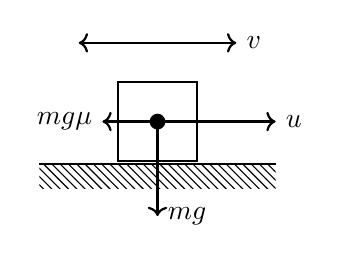
\begin{tikzpicture}
\tikzstyle{ground}=[fill,pattern=north west lines,draw=none,minimum width=2,minimum height=0.5]
\node (wall1) [ground, minimum height=0.3cm, minimum width=3cm] {};
\draw [thick] (wall1.north west) -- (wall1.north east);
\node [draw,minimum width=1cm,minimum height=1cm, thick] (mass) at (0,0.7) {};
\draw [thick, ->] (mass.center) -- +(1.5cm,0cm)  node[right] {$u$};
\draw [thick, ->] (mass.center) -- +(0cm,-1.2cm)  node[right] {$mg$};
\draw [thick, ->] (mass.center) -- +(-0.7cm,0cm)  node[left] {$m g \mu$};
\node [circle, fill=black, inner sep=0cm,minimum size=0.2cm] (b) at (mass) {};
\draw [thick, <->] ($(mass.center)+(-1cm,1cm)$) -- ($(mass.center)+(1cm,1cm)$)  node[right] {$v$};
            \end{tikzpicture}
    \end{figure}
\end{frame}

\begin{frame}
    \frametitle{A simple example (matrix form)}
\[
    0 \leq 
    \underbrace{
    \begin{bmatrix}
        \lambda^+_{k+1} \\
        \lambda^-_{k+1} \\
        \gamma_{k+1}
    \end{bmatrix}
    }_\lambda
    \perp
    \underbrace{
    \begin{bmatrix}
        1 & -1 & 1 \\
        -1 & 1 & 1 \\
        -1 & -1 & 0
    \end{bmatrix}
    }_\text{M}
    \begin{bmatrix}
        \lambda^+_{k+1} \\
        \lambda^-_{k+1} \\
        \gamma_{k+1}
    \end{bmatrix}
    +
    \underbrace{
    \begin{bmatrix}
        v_k + u_{k+1} \\
        -v_k - u_{k+1} \\
        m g \mu
    \end{bmatrix}
    }_\text{q}
    \geq 0
\]
\begin{itemize} 
    \item $M$ is not PSD, but with some small adjustments Anitescu shows Lemke always finds solution
    \item Not necessarily unique
    \item Generalizes to friction cone approximation
\end{itemize}
\end{frame}

\begin{frame}
    \frametitle{Existing approaches}
    \begin{columns}[t]
        \begin{column}{0.33\textwidth}
            \textbf{Learned}
            \begin{itemize}
                \item Often in context of policy learning
                \item Slow and data innefficient
                \item Doesn't leverage existing understanding of contact dynamics
            \end{itemize}
        \end{column}

        \begin{column}{0.33\textwidth}
            \textbf{Hybrid}
            \begin{itemize}
                \item Best of both worlds
                \item Sim-to-real
                \item Residual physics
                \item \textbf{Differentiation through LCPs}
            \end{itemize}
        \end{column}

        \begin{column}{0.33\textwidth}
            \textbf{Analytical}
            \begin{itemize}
                \item Only an approximation
                \item Doesn't fully capture real-world phenomena
            \end{itemize}
        \end{column}
    \end{columns}
\end{frame}

\begin{frame}
    \frametitle{LCP differentiation (Belbute-Peres / Amos / Kolter)}
    \begin{itemize}
        \item Similar to previous work on QPs
            \begin{itemize}
                \item KKT conditions for QP are an LCP
            \end{itemize}
        \item Gives gradients of LCP solutions with respect to $M$ and $q$
        \item Forms bilevel optimization problem:
    \end{itemize}
    \begin{align*}
        \min_{M,q} \quad &\sum_i (\textrm{Dynamics($x_i$,$\lambda_i$)} - \bar{x_i})^2 \\
        \textrm{subject to} \quad &\lambda_i \in LCP(M, q)
    \end{align*}
    \begin{itemize}
        \item \textbf{Problem:} bad priors can cause zero gradients
        \item \textbf{Cause:} hard constriants in LCP
    \end{itemize}
\end{frame}

\begin{frame}
    \frametitle{Reformulating the optimization problem}
    \begin{itemize}
        \item Move cost into subproblem
        \item Soften hard LCP constraints
        \item Allow unphysical behavior to reduce prediction error
    \end{itemize}
    \begin{align*}
        \min_{M,q} \quad &\sum_i c_i \\
        \textrm{subject to} \quad &c_i = \min_{\lambda_i \geq 0} \quad (\textrm{Dynamics($x_i$,$\lambda_i$)} - \bar{x_i})^2\\
                                  & \quad \quad \quad \quad + \lambda_i^T (M \lambda_i + q)
                                                                    + \textrm{hinge}(M\lambda_i + q)
    \end{align*}
\end{frame}

\begin{frame}
    \frametitle{Learning $\mu=1$}
    \begin{figure}
        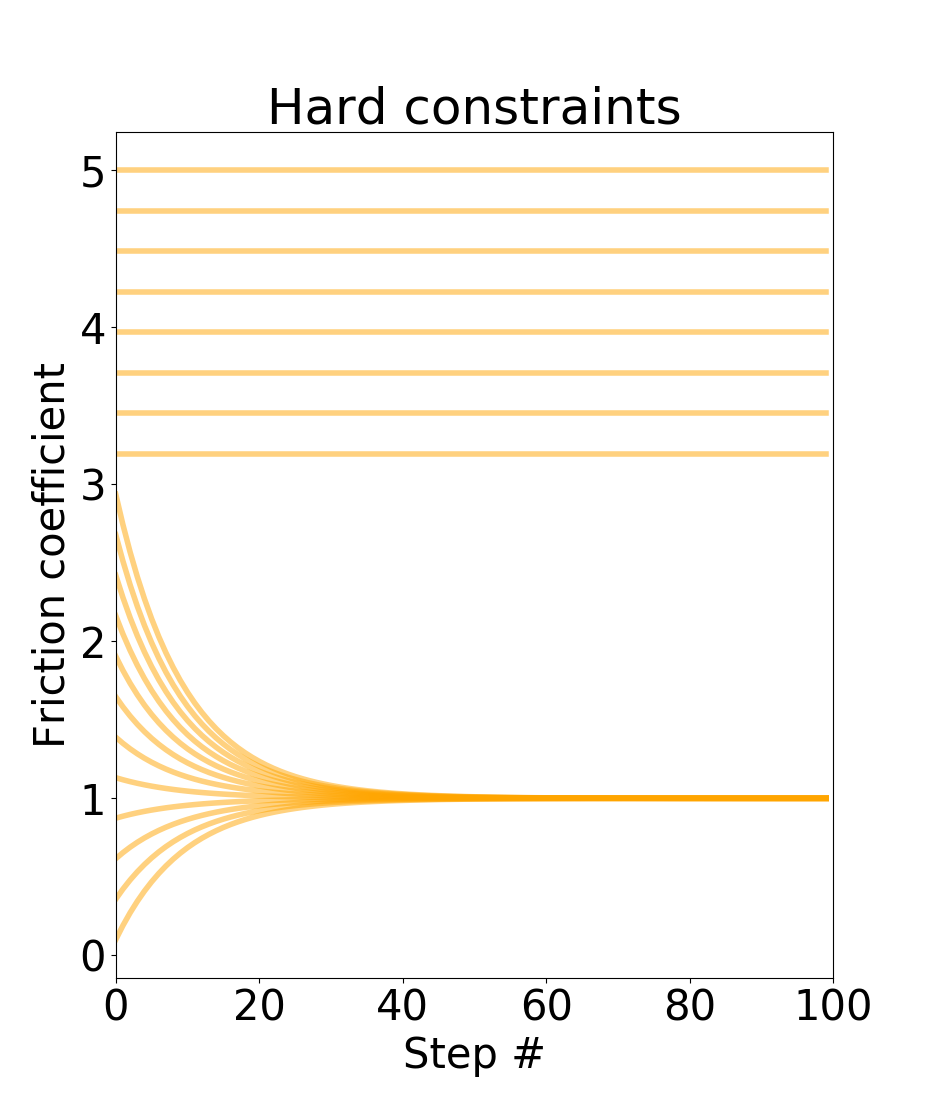
\includegraphics[width=0.5\textwidth]{hard_constraints.png}%
        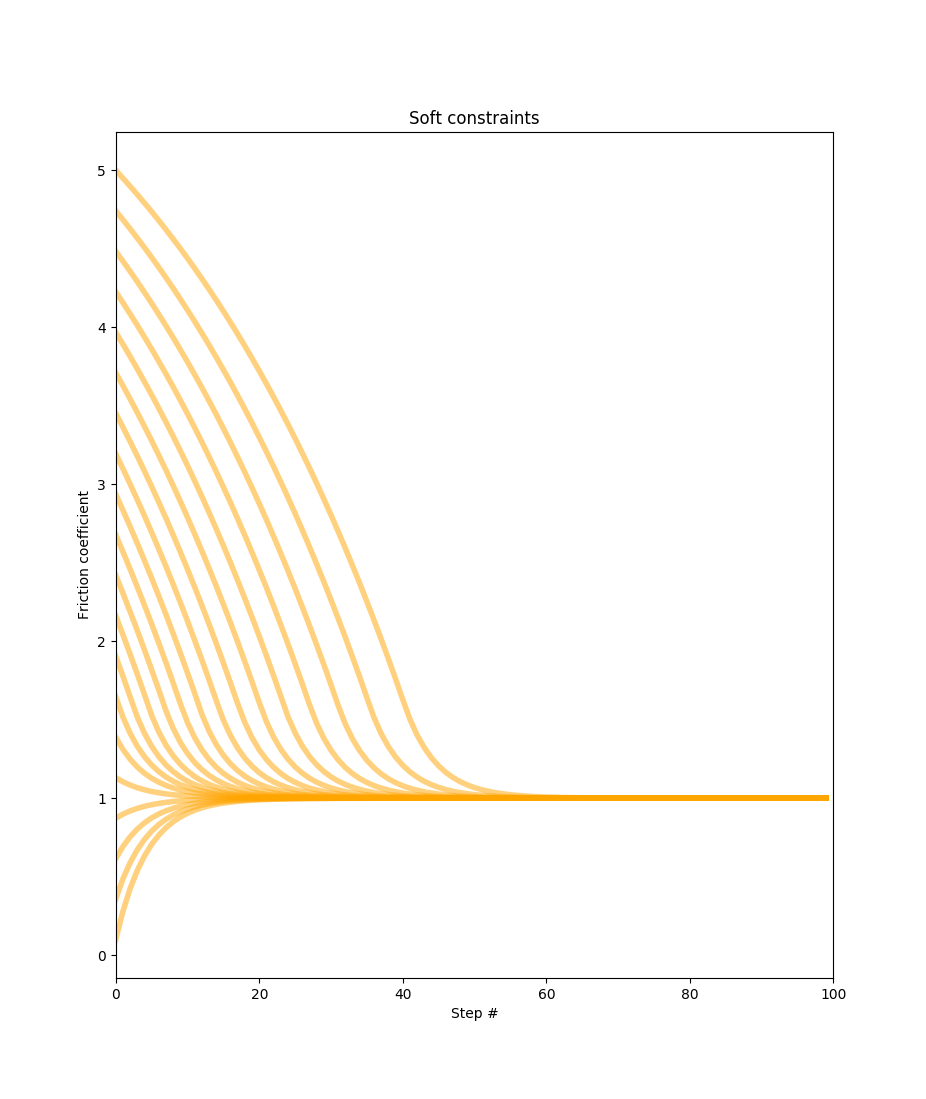
\includegraphics[width=0.5\textwidth]{soft_constraints.png}
    \end{figure}
\end{frame}

\begin{frame}
    \frametitle{The lower level optimization problem}

    \begin{itemize}
        \item Can be written in quadratic form:
    \end{itemize}
\begin{align*}
    (\textrm{Dynamics($x_i$,$\lambda_i$)} - \bar{x_i})^2 = &\left(v_{k + 1} - (v_k + \lambda^+_i - \lambda^-_i + u_i)\right)^2 \\
  &\textrm{Write $\beta_i = v_{k+1} - v_k - u_i$: } \\
    = &\lambda_i^T 
        \underbrace{
            \begin{bmatrix} 1 & -1 & 0 \\ -1 & 1 & 0 \\ 0 & 0 & 0 \end{bmatrix} 
        }_D
        \lambda_i + \underbrace{
            \begin{bmatrix} -2 \beta_i & 2 \beta_i & 0 \end{bmatrix}
        }_b  \lambda_i 
\end{align*}
    
    \begin{itemize}
        \item Get lower-level QP (with hard nonnegativity constraint):
    \end{itemize}
    \begin{align*}
        \min _{\lambda_i \geq 0} \quad & \frac{1}{2} \lambda_i^T (Q + Q^T)  \lambda_i + (q^T + b) \lambda_i \\
                                       &M \lambda_i + q \geq 0 \\
                                       & Q = M + D
    \end{align*}
\end{frame}

\begin{frame}
    \frametitle{Convexity guarantees}
    \begin{itemize}
        \item Want symmetric part of $M + D$ to have nonnegative eigenvalues
        \item Eigenvalues of $D$ nonnegative, real
        \item Eigenvalues of $M$ complex with nonnegative real part
        \item Extend analysis to full Anitescu formulation
        \item Scaling $D$ with sufficiently large constant?
    \end{itemize}
\end{frame}

\begin{frame}
    \frametitle{Structured learning}
    \begin{itemize}
        \item Elementwise learning of $M$, $q$ undesirable
        \begin{itemize}
            \item Can prove an $\epsilon$ error in single $q$ element breaks sticking
            \item Coefficient antisymmetry across rows breaks sticking
        \end{itemize}
        \item How much structure do we need to impose?
        \begin{itemize}
            \item Learning physical parameters intuitive but restrictive
            \item Eventually progress to noninterpretable parameters 
        \end{itemize}
    \end{itemize}
\end{frame}

\begin{frame}[plain,c]
    \frametitle{Thank you!}
    \begin{enumerate}
        \small
        \item Anitescu, M., and F. A. Potra. ``Formulating Dynamic Multi-rigid-body Contact Problems with Friction as Solvable Linear Complementarity Problems." (1996).
        \item Stewart, David, and Jeffrey C. Trinkle. ``An implicit time-stepping scheme for rigid body dynamics with coulomb friction." Proceedings 2000 ICRA. Millennium Conference. IEEE International Conference on Robotics and Automation. Symposia Proceedings (Cat. No. 00CH37065). Vol. 1. IEEE, 2000. 
        \item de Avila Belbute-Peres, Filipe, et al. ``End-to-end differentiable physics for learning and control." Advances in Neural Information Processing Systems. 2018. 
        \item Amos, Brandon, and J. Zico Kolter. ``Optnet: Differentiable optimization as a layer in neural networks." Proceedings of the 34th International Conference on Machine Learning-Volume 70. JMLR. org, 2017. 
    \end{center}
\end{frame}

\end{document}
